\begin{table}[ht]
\centering
\begin{tabular}{lrrrrr}
\toprule
Target B &     A &     B &      C &     D &     E \\
Source &       &       &        &       &       \\
\midrule
A      &  8,833 &   430 &    709 &     1 &     0 \\
B      &   249 &  6,710 &    536 &   526 &   681 \\
C      &   925 &   552 &  19,275 &     5 &     0 \\
D      &     0 &   326 &      2 &  7,906 &   314 \\
E      &     0 &   382 &      0 &   742 &  7,523 \\
\bottomrule
\end{tabular}
\caption{Confusion table showing branch labels of the optimal matches of cells in the simulated PROSST data, between Source and Target B. Entries on the diagonal correspond to correct matches whereas off-diagonal elements to mismatches. The overall accuracy, with respect to the branch label, equals 89\%.}
\label{tbl:prosstt_conf_SB}
\end{table}

\begin{table}
\centering
\begin{tabular}{lrrrrr}
\toprule
Target B &     A &     B &      C &     D &     E \\
Target A &       &       &        &       &       \\
\midrule
A      &  7,718 &   738 &    844 &    21 &    19 \\
B      &   518 &  6,312 &    785 &   679 &  1190 \\
C      &   777 &   865 &  18,460 &    20 &    42 \\
D      &    83 &   469 &     36 &  8,054 &   248 \\
E      &    25 &   904 &     66 &   517 &  7,232 \\
\bottomrule
\end{tabular}
\caption{Confusion table showing branch labels of the optimal matches of cells in the simulated PROSST data, between Target A and Target B. Entries on the diagonal correspond to correct matches whereas off-diagonal elements to mismatches. The overall accuracy, with respect to the branch label, equals 84\%.}
\label{tbl:prosstt_conf_AB}
\end{table}

\begin{figure}[htb]
    \centering
    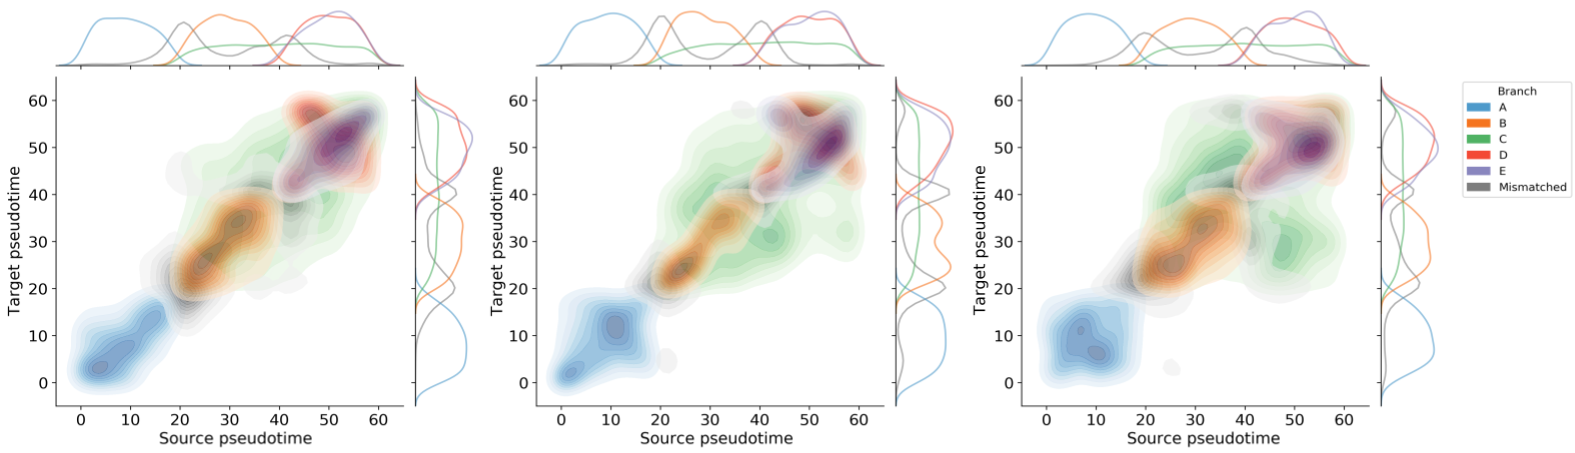
\includegraphics[width=1\textwidth]{figures/integration/3tech-pseudotime-kde.png}
    \caption{
    Evaluation of cross-technology cell matches made by SCIM on the simulated data with three technologies. 
    The pairwise matching is attained for Source-Target A, Source-Target B, and Target A-Target B, respectively. The sink edge capacities were unbounded in all cases.
    Here, we show a density plot for matched pseudotime values between the source technology and the target technology,
    colored by the branch label. Mismatched cells are colored in grey.
    The tree defining the temporal branching process can be found in Figure \ref{}, left.
    Marginal distributions of cell pseudotime for each branch is shown on the top and right.
    }
    \label{fig:prosstt5-3tech-pseudotime}
\end{figure}

\begin{table}
\centering
\begin{tabular}{l|llllll}
\toprule
  method & accuracy & \#null matches & Spearman & Pearson \\
\midrule
 SCIM    &   86\% &  1,590  & 0.83  & 0.86\\
 MATCHER &   4\%  & 25,510  & -0.21 & -0.19\\
\bottomrule
\end{tabular}
\caption{The matching results on the PROSSTT dataset, where the SCIM matching algorithm was applied to SCIM shared latent codes and the MATCHER latent representation. The table depicts accuracy with respect to branch label, null node matches and the correlation coefficients for the pseudotime between matched source and target cells.}
\label{tbl:prosstt_matcher}
\end{table}

\begin{figure}[htp]
    \centering
    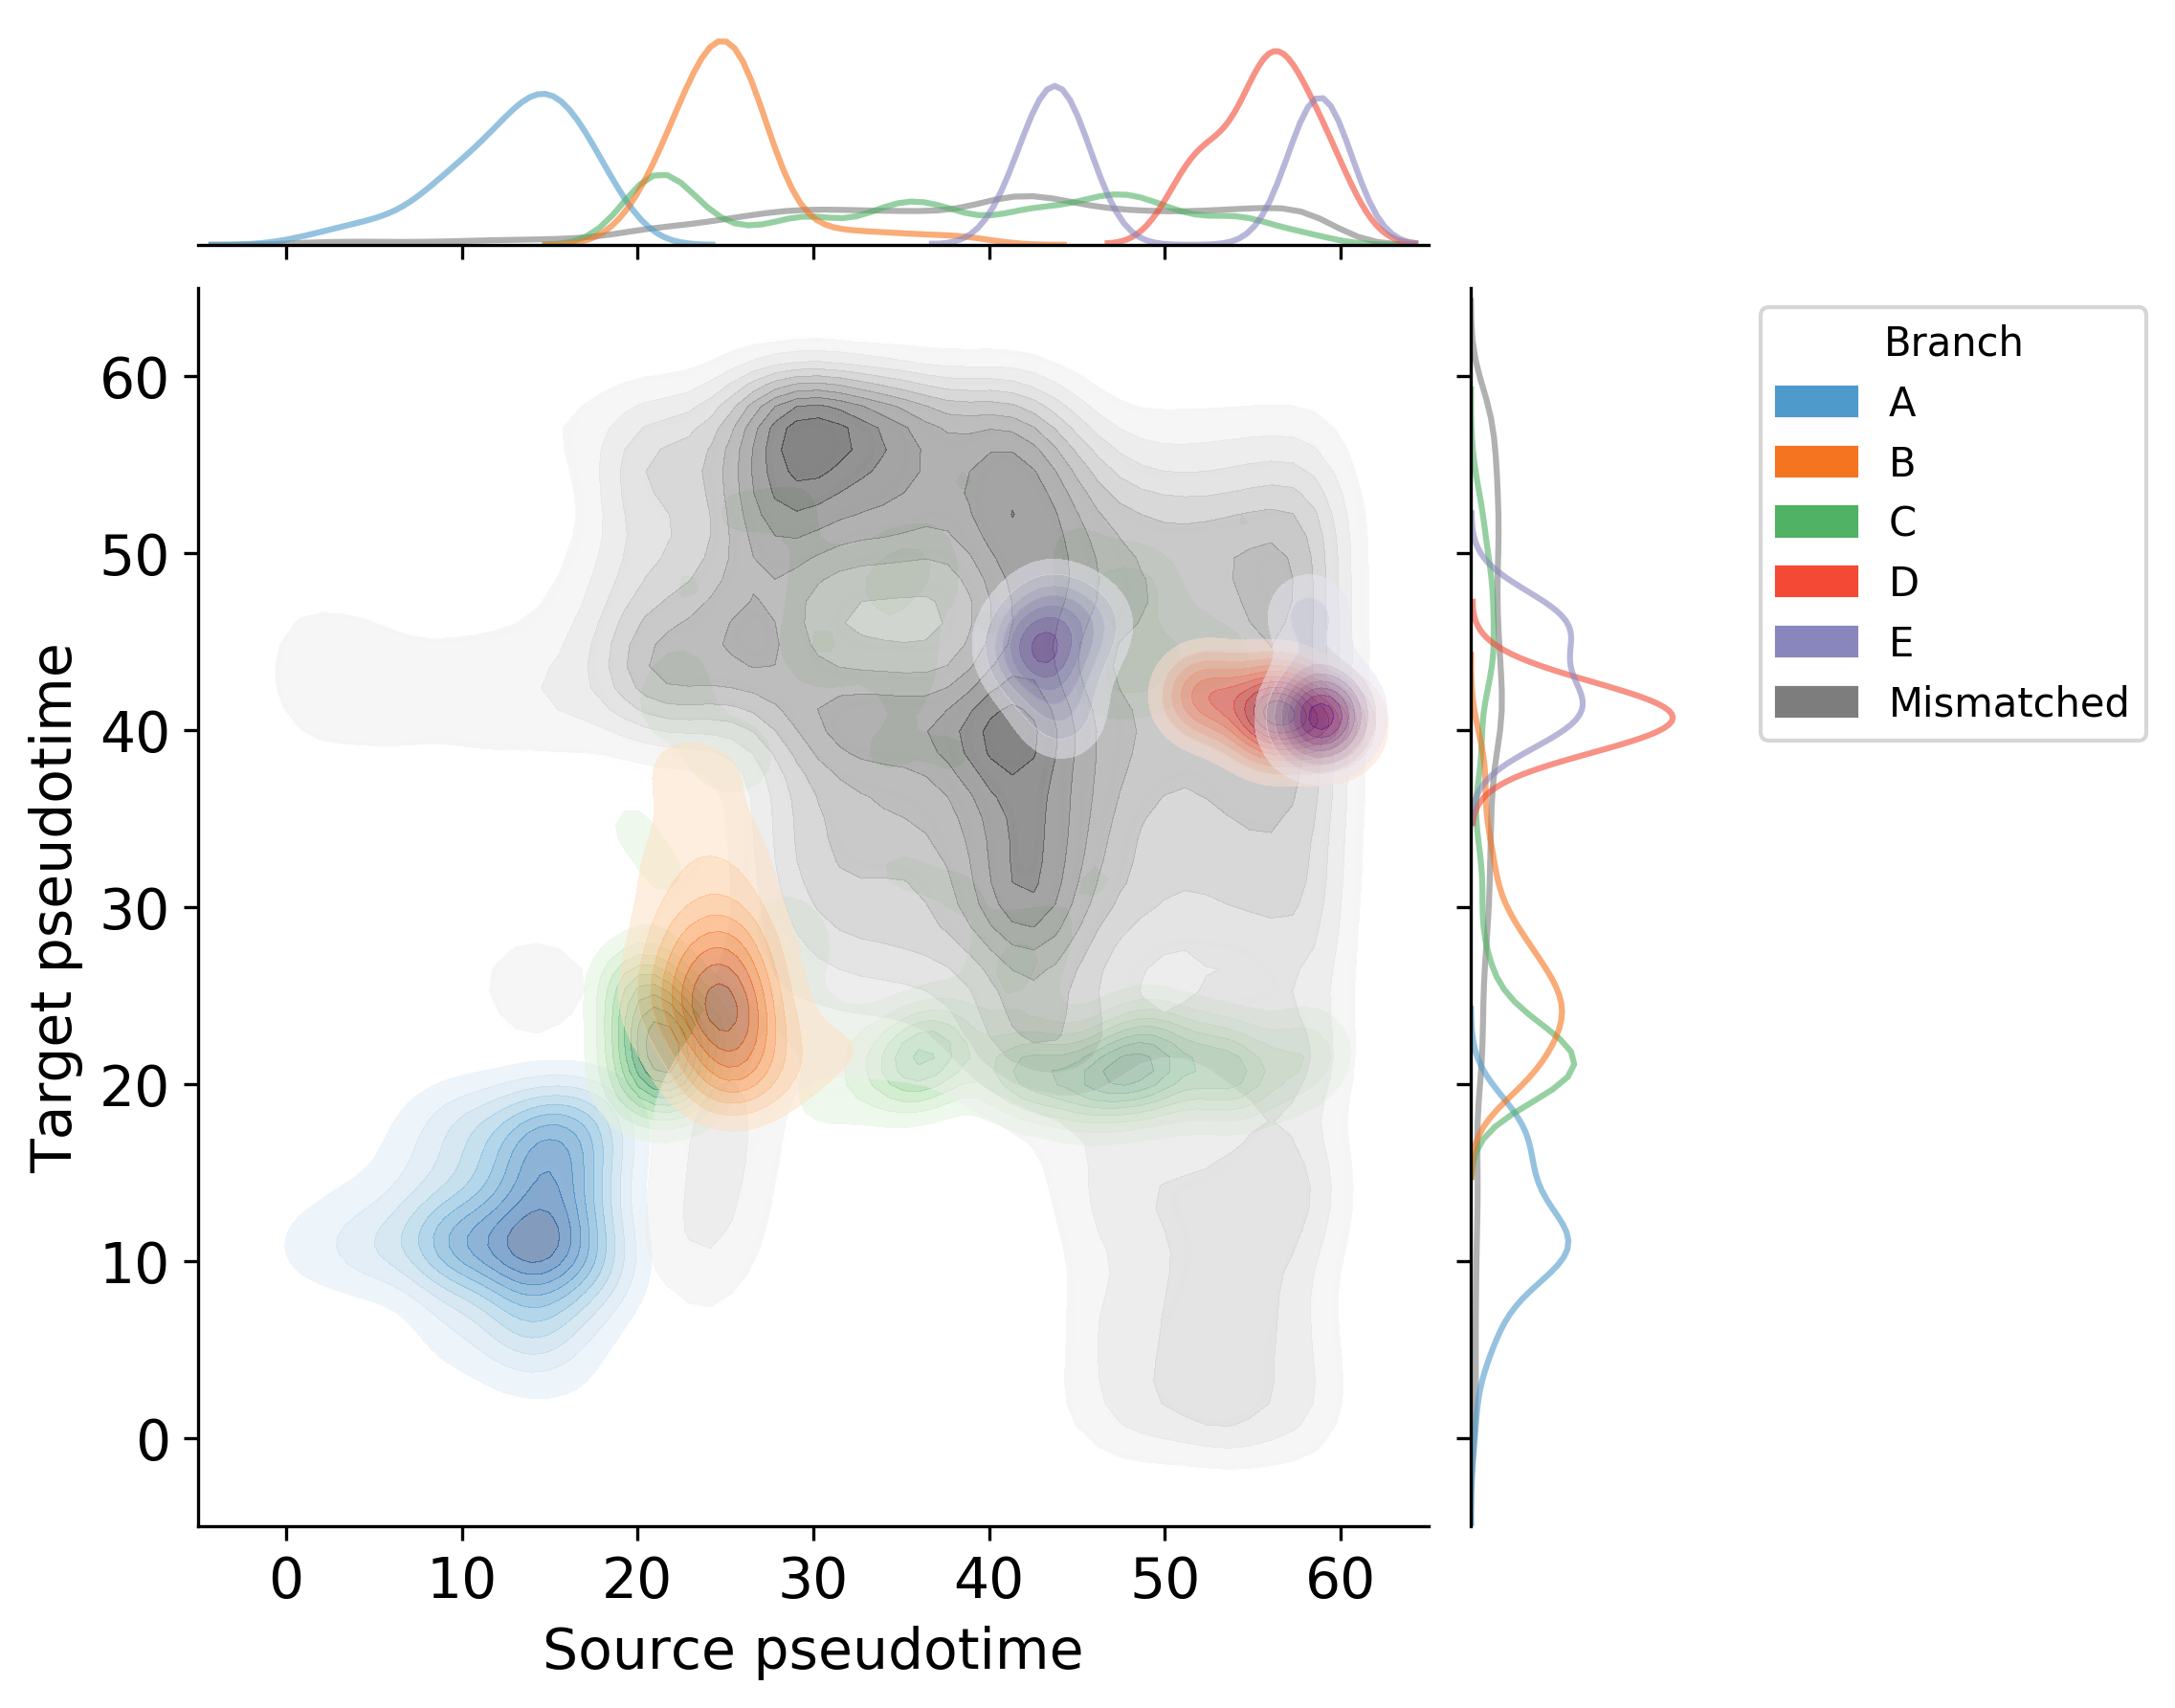
\includegraphics[width=1.0\textwidth]{figures/integration/matcher-pseudotime-kde.png}
    \caption{
    Evaluation of cross-technology cell matches using latent representation obtained by MATCHER on the simulated data.
    Cells are matched across datasets pairwise using the bipartite matching scheme.
    Here we show a density plot for matched pseudotime values between the source technology and the target technology,
    colored by the branch label. Mismatched cells are colored in grey.
    Marginal distributions of cell pseudotime for each branch are shown on the top and right.
    }
    \label{fig:prosstt5-matcher-psuedotime}
\end{figure}

\begin{figure}[htbp]
    \centering
    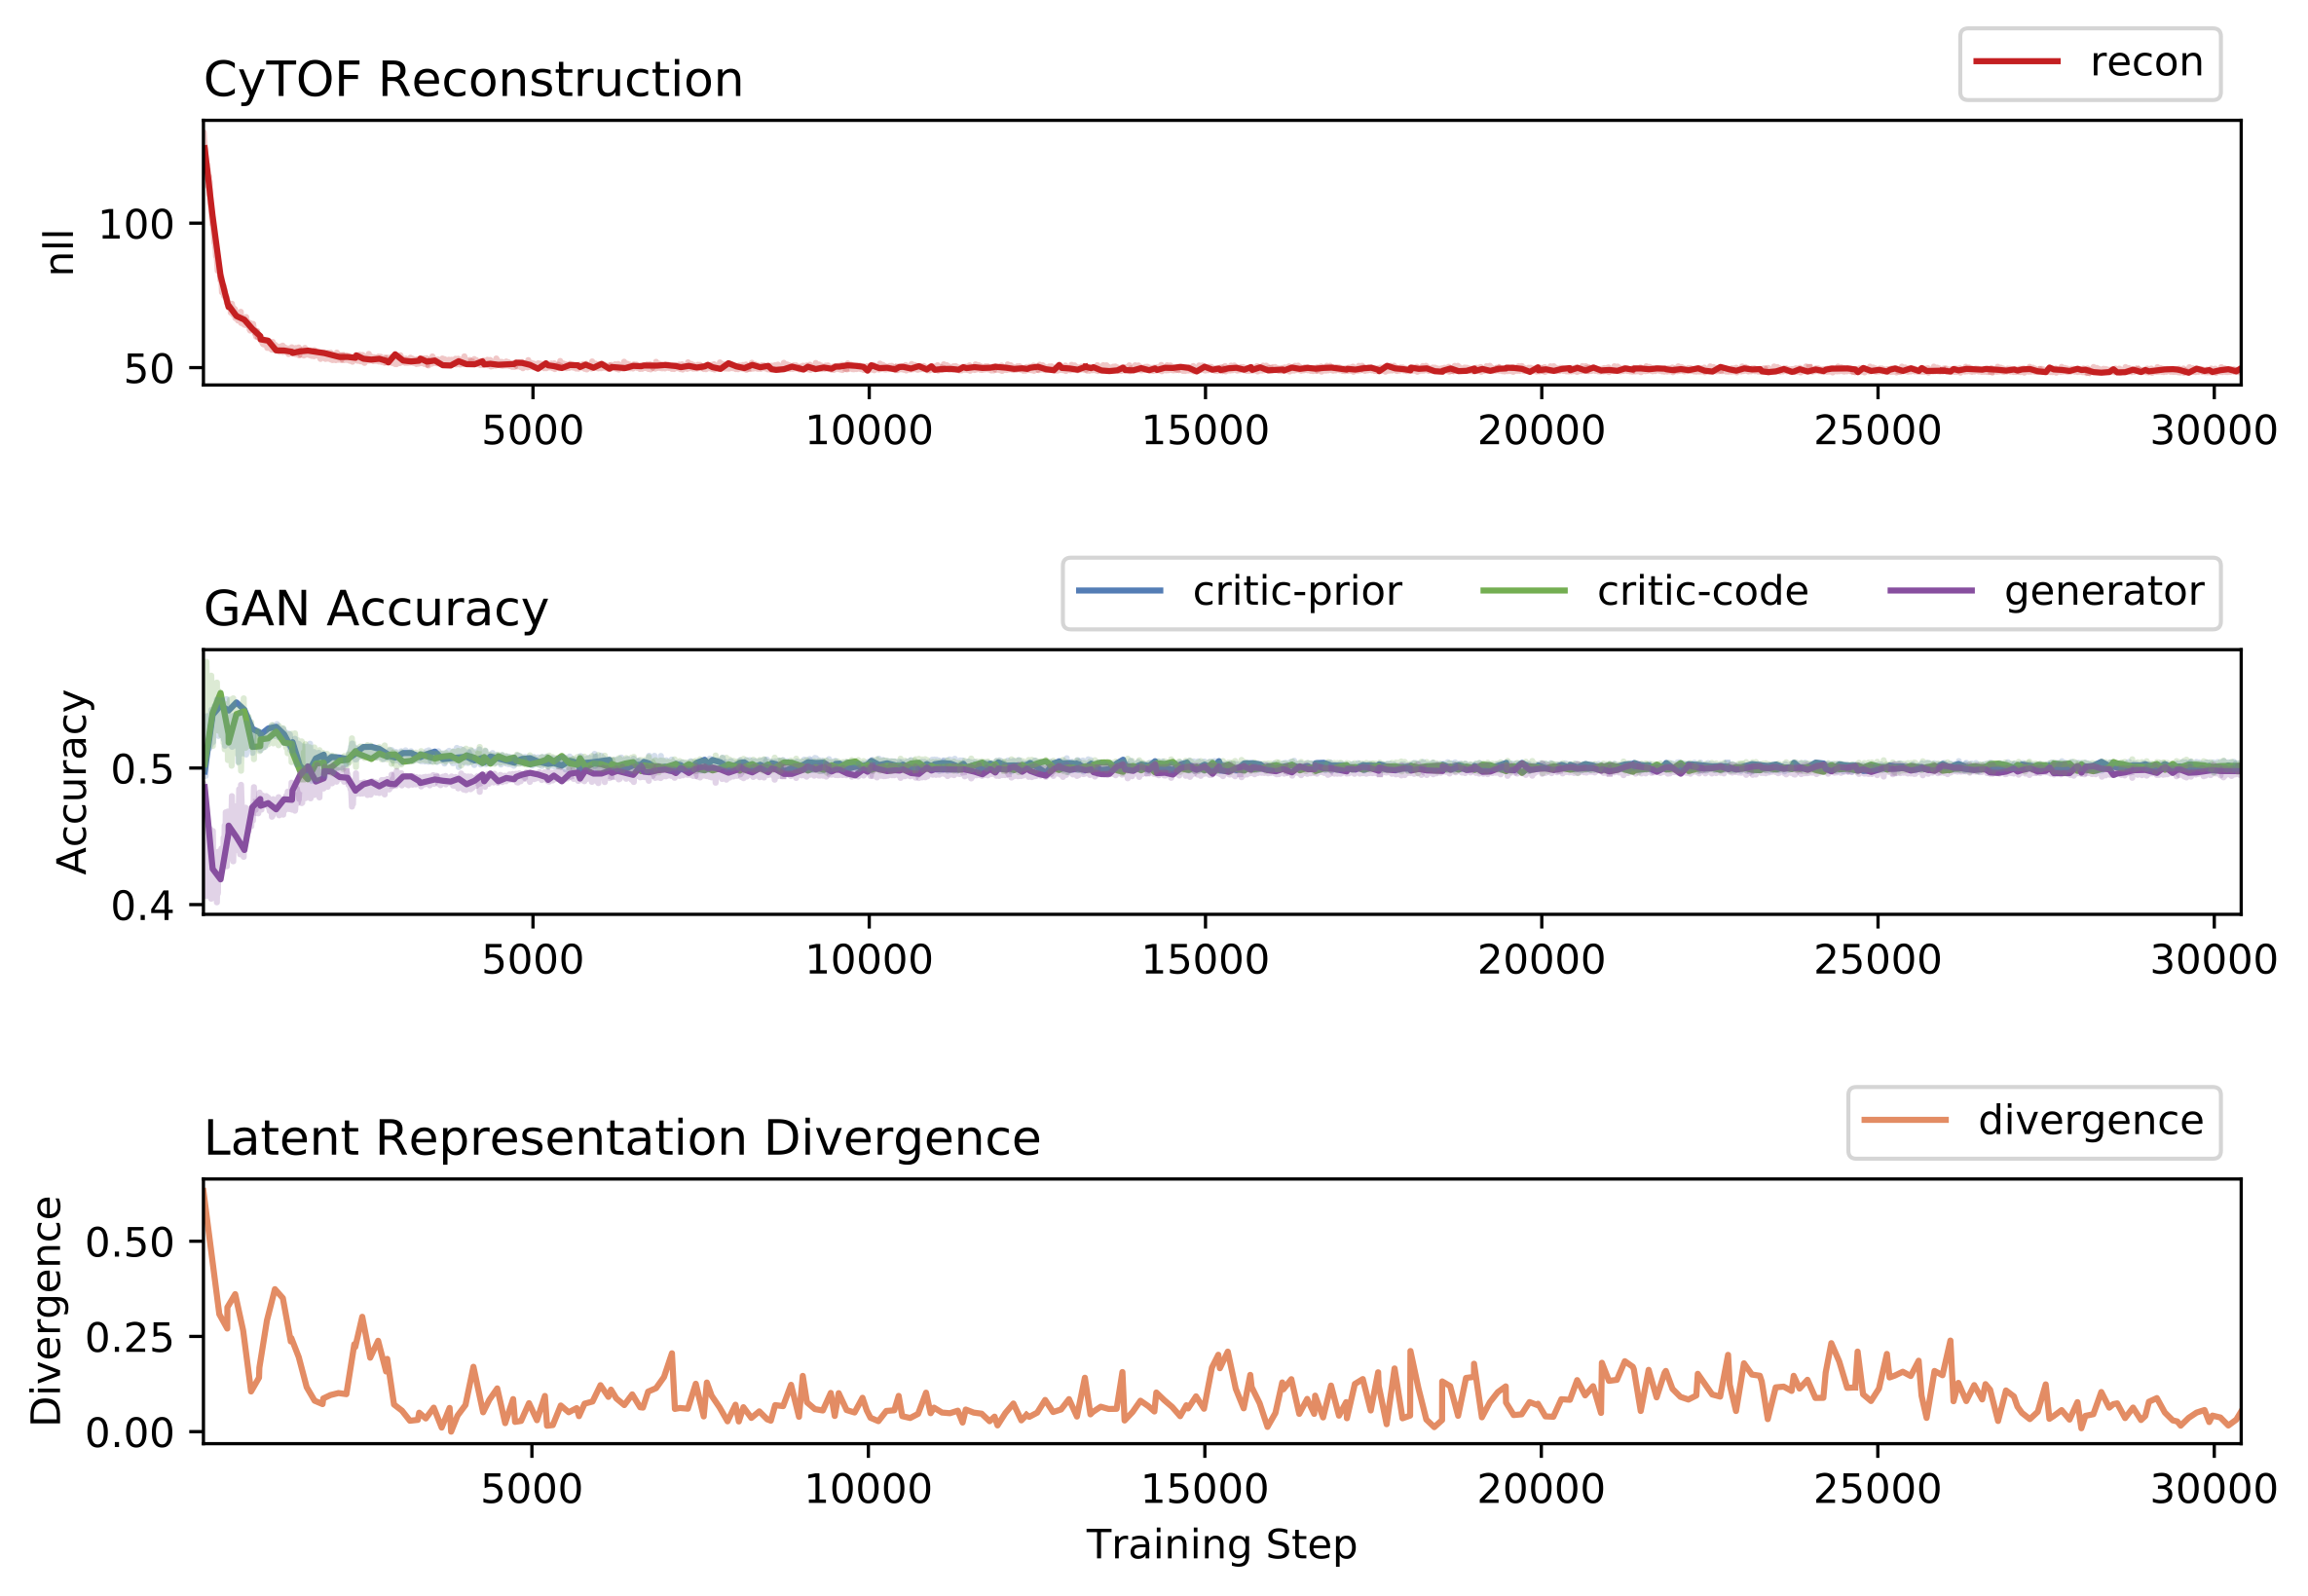
\includegraphics[width=0.95\textwidth]{figures/integration/menytek-train-scores}
    \caption{
        Training progress of SCIM on a melanoma sample.
        The latent space is initialized by training a VAE on scRNA data.
        SCIM integrates CyTOF representations into the latent space
        defined by the scRNA codes.
        The top panel shows the negative log-likelihood of the CyTOF reconstruction.
        The middle panel shows the performance of the discriminator to correctly classify scRNA codes (critic-prior), CyTOF codes (critic-code), and the ability of the encoder to fool the discriminator, i.e., the misclassification accuracy (generator).
        The bottom panel shows the divergence of the latent representations.
        The model is able to converge quickly.
However, the divergence score can fluctuate despite still fooling the discriminator.
        Training took 2h 10min and had a peak memory consumption of 1068 MB.
    }
    \label{fig:tupro-train}
\end{figure}


\begin{table}[h]
\centering
\begin{tabular}{rrrrrr}
\toprule
Censor & $\beta$ &  ${lr}_{\phi,\psi}$&  ${lr}_\gamma$ & Success &  \# runs \\
\midrule
0.00 &      16 &            0.0010 &  0.0010 &         14\% &           7 \\
     &      16 &            0.0010 &  0.0005 &         14\% &           7 \\
     &      16 &            0.0005 &  0.0005 &         10\% &          10 \\
     &      16 &            0.0005 &  0.0010 &         10\% &          10 \\
0.25 &      16 &            0.0010 &  0.0010 &         14\% &          14 \\
     &      16 &            0.0005 &  0.0010 &         12\% &          17 \\
     &      64 &            0.0001 &  0.0005 &          0\% &           7 \\
     &      64 &            0.0001 &  0.0010 &          0\% &           7 \\
0.75 &      16 &            0.0005 &  0.0010 &         17\% &           6 \\
     &      32 &            0.0005 &  0.0005 &         12\% &           8 \\
     &      16 &            0.0010 &  0.0005 &          8\% &          13 \\
     &      64 &            0.0001 &  0.0005 &          0\% &           7 \\
0.90 &      16 &            0.0005 &  0.0010 &         40\% &          10 \\
     &      16 &            0.0010 &  0.0005 &         10\% &          10 \\
     &      16 &            0.0005 &  0.0005 &          8\% &          12 \\
     &      32 &            0.0010 &  0.0001 &          0\% &          10 \\
0.95 &      32 &            0.0010 &  0.0001 &          0\% &           4 \\
     &      64 &            0.0001 &  0.0005 &          0\% &           4 \\
     &      64 &            0.0001 &  0.0010 &          0\% &           6 \\
     &      32 &            0.0010 &  0.0010 &          0\% &           5 \\
0.99 &      16 &            0.0005 &  0.0010 &         17\% &           6 \\
     &      32 &            0.0010 &  0.0005 &          0\% &           6 \\
     &      64 &            0.0001 &  0.0005 &          0\% &           4 \\
     &      32 &            0.0010 &  0.0001 &          0\% &           6 \\
\bottomrule
\end{tabular}
\caption{
    Ablation study for training SCIM on the melanoma patient at several levels of semi-supervision.
    Fraction censored is the fraction of labels removed during training.
    The top 4 configurations for each level of semi-supervision is shown.
    $\beta$ is the regularization strength of the adversarial loss.
    Learning rates are the initial settings of the ADAM optimizer.
    If the latent space divergence is below 0.3 and
    the negative log-likelihood of the input under the reconstruction is below 47,
    the training is determined to be a success. These values were chosen empirically.
    We see that $\beta$ and optimizer learning rates were heavily influential on model success.
}
\label{tbl:ablation_menytek}
\end{table}

\begin{figure}[h]
    \centering
    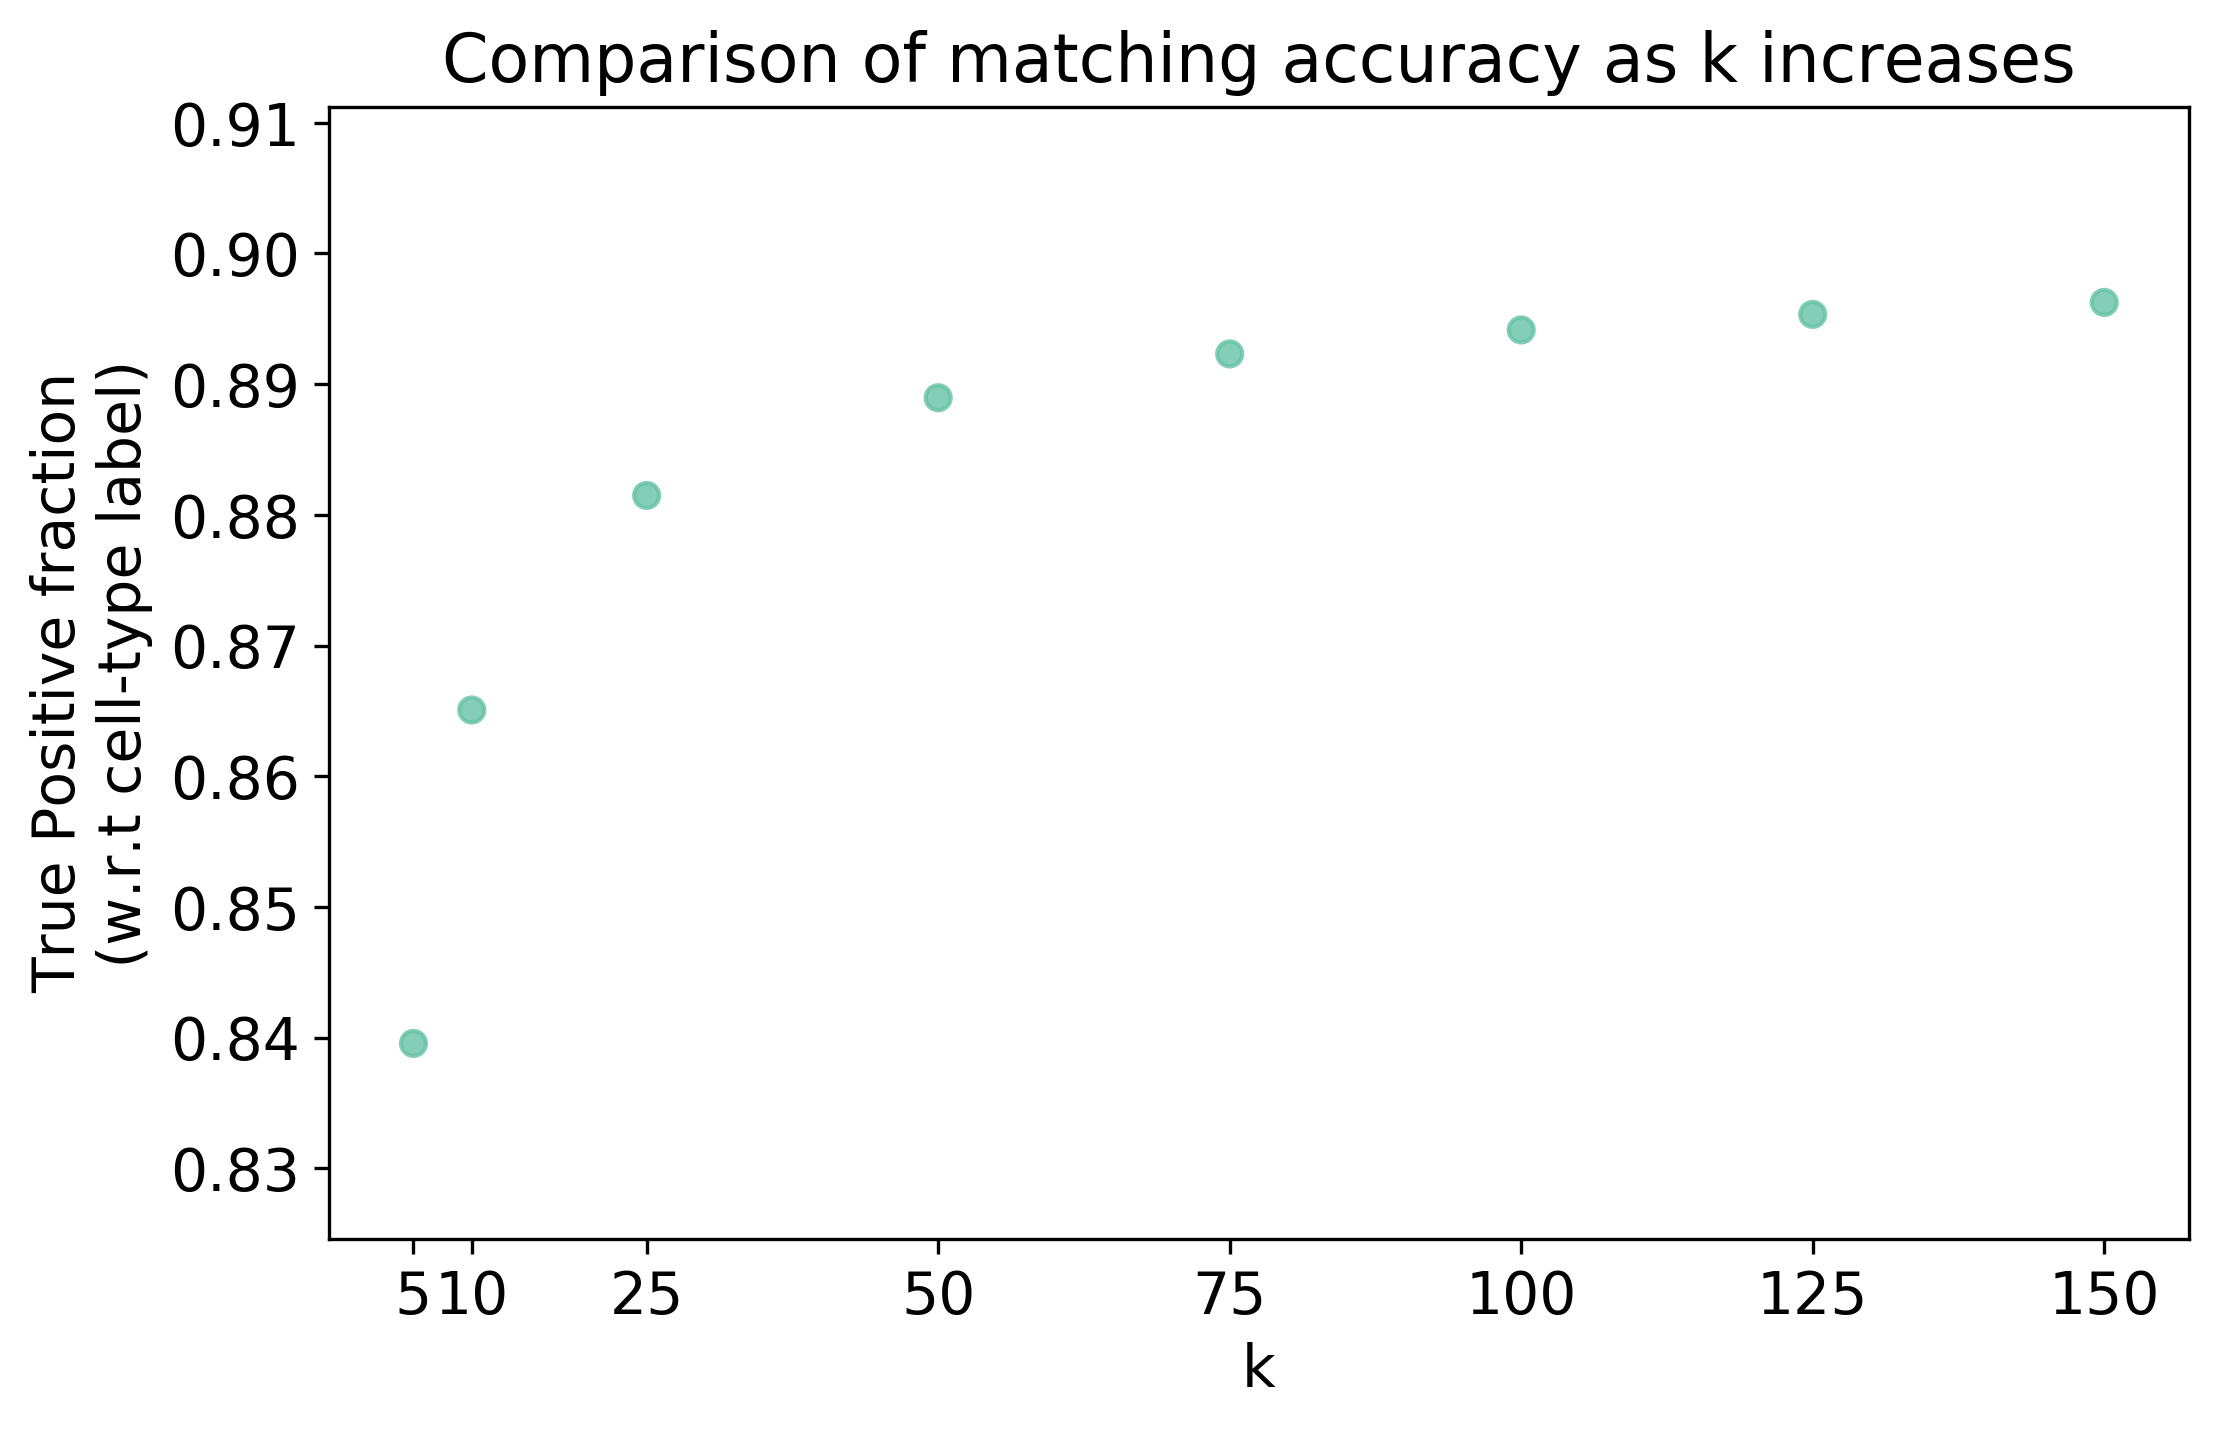
\includegraphics[width=0.85\textwidth]{figures/integration/matching-tune-k-unicapacity.png}
    \caption{Comparison of matching accuracy, with respect to cell-type label as less sparsity of connections, is imposed on the Tumor Profiler data.
The number of considered Nearest Neighbors \textit{k} is indicated on the x-axis, and the fraction of true positive matches, with respect to cell-type label, is depicted on the y-axis.
 The accuracy level saturates with $k=100$.}
    \label{fig:matching_accuracy_log10_uni}
\end{figure}

\begin{table}[h]
\centering
\begin{tabular}{lrr}
\toprule
{} &  CPU time [s] &  Max Memory [Mb] \\
k   &               &                  \\
\midrule
5   &       1,492.67 &          1,674.94 \\
10  &       2,803.33 &          2,456.27 \\
25  &       7,723.67 &          4,690.05 \\
50  &       7,441.33 &          8,740.34 \\
75  &      12,656.00 &         12,344.52 \\
100 &      17,331.00 &         17,002.75 \\
125 &      26,047.00 &         20,612.78 \\
150 &      33,718.00 &         24,222.75 \\
\bottomrule
\end{tabular}
\caption{Memory usage and computation time of the bipartite matching as \textit{k} hyperparameter in kNN search increases.
The values were obtained on the whole TuPro dataset using the MCMF algorithm on an extended graph. %, as described in section \ref{graph_extensions}.
The cost of matching to the null node was set to 95th percentile, and a union of connections obtained from kNN graphs with \textit{k} indicated in the first column was used for matching.
The memory and time reports were averaged across three independent runs.}
\label{tbl:menytek_tune_k_uni}
\end{table}

\begin{figure}[htbp]
    \centering
    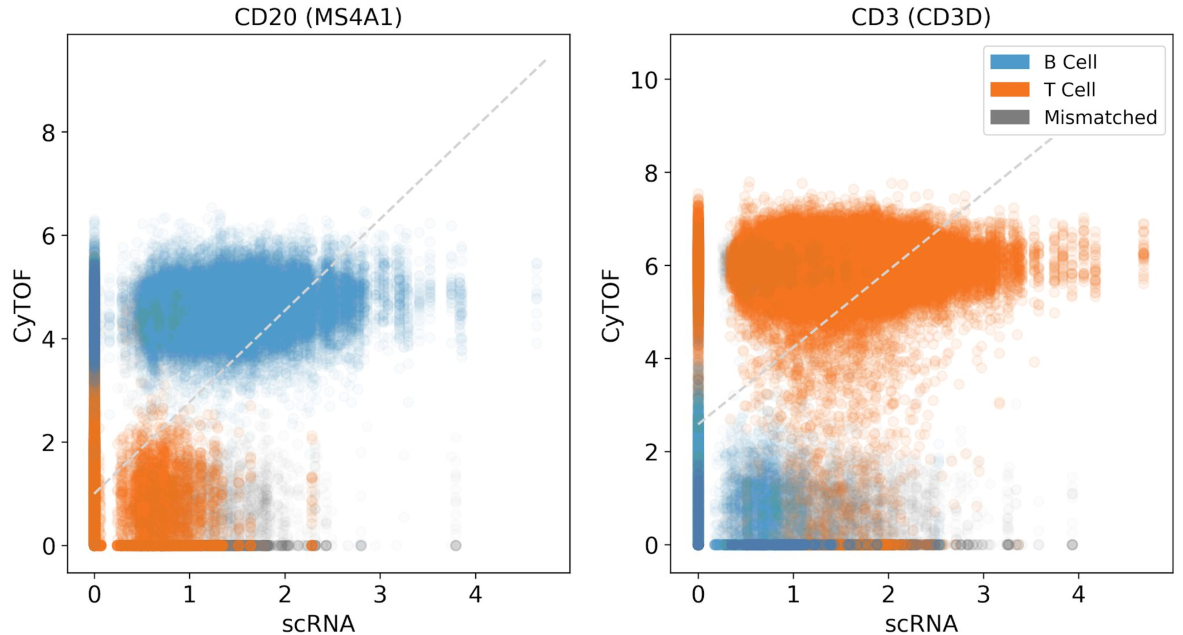
\includegraphics[width=0.65\textwidth]{figures/integration/gene_protein_correlation_unicapacity}
    \caption{
      \textit{CD20} and \textit{CD3} marker abundances measured with scRNA (gene, x-axis) and CyTOF (protein, y-axis) in a melanoma sample from the Tumor Profiler Consortium.
      The values on the axes represent normalized expression.
      Colors (blue, orange) represent cell types (B-cell, T-cell) while grey marks mismatches with respect to the cell-type label.
      The linear regression line is depicted by a dashed light grey line.
      Pearson's correlation coefficient equals 0.63 and 0.51 for CD20 and CD3, respectively.
      Spearman's correlation coefficient amounts to 0.55 and 0.42, for CD20 and CD3, respectively.
    }
    \label{fig:tupro-marker-correlation-uni}
\end{figure}

\begin{figure}[htb]
    \centering
    \includegraphics[width=0.85\textwidth]{figures/integration/oetjen-tsne-matched-unicapacity.png}
    \caption{
    A tSNE embedding (perplexity=30) of the integrated latent space with cell matches indicated by the grey lines.
    The shared representation was obtained in a semi-supervised fashion, utilizing 10\% of the cell-type labels to orient the latent space. 10,000 matched pairs were sampled at random for the plot.
    Colors (blue, green, orange) represent T-cell subtypes (CD8 effector, CD4 naive, CD4 memory), and color shades correspond to the profiling technology (light: scRNA, dark: CyTOF).}
    \label{fig:oetjen_tsne_uni}
\end{figure}
